\documentclass[11pt,a4paper]{article}
\usepackage[a4paper, hmargin={2.5cm,2.5cm},vmargin={2.5cm,2.5cm}]{geometry}
\usepackage{graphicx}
\usepackage{cmap}
\usepackage[utf8]{inputenc}
\usepackage[english]{babel}
\usepackage{amsmath}
\usepackage{amsfonts}
\usepackage{listings}
\usepackage{color}
\usepackage{pdfpages}
\usepackage{fancyvrb}
\usepackage{fancyhdr}
\usepackage{lipsum}
% \usepackage{pgfplots}
\usepackage{hyperref}
\usepackage{subfig}
\usepackage{enumitem}
\usepackage{tikz}
\usepackage{forest}

\usetikzlibrary{automata, positioning, arrows}
\usetikzlibrary{positioning}
\usetikzlibrary{shapes,shapes.geometric,arrows,fit,calc}


\def\dunderline#1{\underline{\underline{#1}}}
\def\indent{\space\space\space\space}
\newcommand\drawloop[4][]%
   {\draw[shorten <=0pt, shorten >=0pt,#1]
      ($(#2)!\pgfkeysvalueof{/tikz/stretch}!(#2.#3)$)
      let \p1=($(#2.center)!\pgfkeysvalueof{/tikz/stretch}!(#2.north)-(#2)$),
          \n1= {veclen(\x1,\y1)*sin(0.5*(#4-#3))/sin(0.5*(180-#4+#3))}
      in arc [start angle={#3-90}, end angle={#4+90}, radius=\n1]%
   }

\definecolor{bluekeywords}{rgb}{0.13,0.13,1}
\definecolor{greencomments}{rgb}{0,0.5,0}
\definecolor{turqoisenumbers}{rgb}{0.17,0.57,0.69}
\definecolor{redstrings}{rgb}{0.5,0,0}

\lstdefinelanguage{FSharp}
  {morekeywords={let, new, match, with, rec, open, module, namespace, type, of, member, and, for, in, do, begin, end, fun, function, try, mutable, if, then, else, rule, \%token},
    keywordstyle=\color{bluekeywords},
    sensitive=false,
    morecomment=[l][\color{greencomments}]{///},
    morecomment=[l][\color{greencomments}]{//},
    morecomment=[s][\color{greencomments}]{{(*)}},
    morestring=[b]",
    stringstyle=\color{redstrings}
    }

\lstset{language=fsharp}


\begin{document}
\begin{titlepage}
    \title{Programmer som data exam}
    \author{Albert Ross Johannessen}
    \maketitle
    \fbox{
      \begin{minipage}{40em}
          \textbf{Jeg erklærer hermed at jeg selv har lavet hele denne eksamensbesvarelse uden hjælp fra andre.}
      \end{minipage}
      }
  \end{titlepage}
  
\pagestyle{fancy}
\fancyhf{}
\rhead{Programmer som data}
\rfoot{Page \thepage}
\section{Opgave 1}
Betragt dette regulære udtryk over alfabetet $\{k,l,v,h,s\}$:
\begin{align*}
    k(l|v|h|)+s
\end{align*}
Ved antagelse, at
\begin{align*}
    k & \text{ svarer til } & kør\\
    l & \text{ svarer til } & ligeud\\
    v & \text{ svarer til } & venstre\\
    h & \text{ svarer til } & højre\\
    s & \text{ svarer til } & slut
\end{align*}
så beskriver det regulære udtryk strenge, der symboliserer køreture, eksempelvis turen fra hjem til ITU.\@
\subsection{Giv nogle eksempler på strenge der genkendes af det regulære udtryk samt en uformel beskrivelse}
Nogle eksempler på strenge der genkendes af det regulære udtryk er.
\begin{itemize}
    \item kls
    \item klllllllls
    \item klvhs
    \item khhhhs
\end{itemize}
Sproget beskriver en mængde handlinger man skal tage på en køretur, man kan enten køre ligeud til venstre eller højre, der er følgende krav til en streng.
\begin{itemize}
    \item Man skal starte med $k$ og slutte med $s$
    \item Mellem $k$ og $s$ skal man \textit{mindst} een gang enten dreje eller køre ligeud.
\end{itemize}
\subsection{Lav udtrykket om til en NFA}
Vi kan starte med at dele udtrykket op i mindre dele og repræsentere dem via en graf visning.\\
\begin{figure}[!ht]
    \centering
    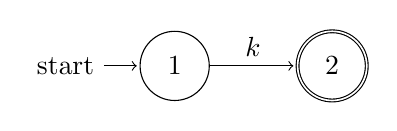
\begin{tikzpicture}[shorten >=1pt,node distance=2cm,on grid,auto] 
       \node[state, initial] (q_1)   {$1$}; 
        \node[state,accepting] (q_2) [ right =of q_1] {$2$};
              
        \path[->] 
        (q_1) edge  node {$k$} (q_2)
        ;
    \end{tikzpicture}
    \caption{$k$}\label{fig:examfignfak}
\end{figure}
\newpage
\begin{figure}[!ht]
    \centering
    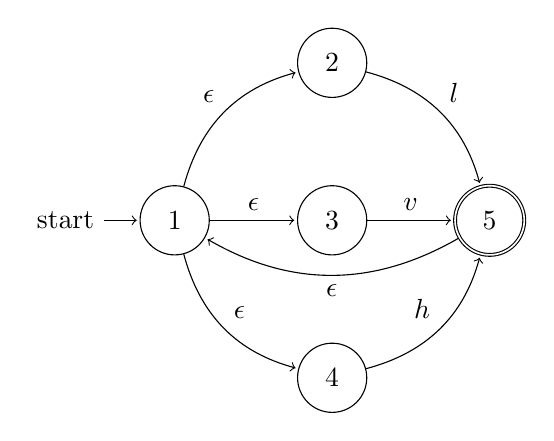
\begin{tikzpicture}[shorten >=1pt,node distance=2cm,on grid,auto] 
       \node[state, initial] (q_1)   {$1$}; 
        \node[state] (q_3) [ right =of q_1] {$3$};
        \node[state] (q_2) [above  =of q_3] {$2$};
        \node[state] (q_4) [below  =of q_3] {$4$};
        \node[state,accepting] (q_5) [ right =of q_3] {$5$};
              
        \path[->] 
        (q_1) edge [bend left] node {$\epsilon$} (q_2)
        (q_1) edge  node {$\epsilon$} (q_3)
        (q_1) edge [bend right] node {$\epsilon$} (q_4)
        (q_2) edge [bend left] node {$l$} (q_5)
        (q_3) edge  node {$v$} (q_5)
        (q_4) edge [bend right] node {$h$} (q_5)
        (q_5) edge [bend left=30] node {$\epsilon$} (q_1)
        ;

    \end{tikzpicture}
    \caption{$(l|v|h)+$}\label{fig:examfignfalvh}
\end{figure}
\begin{figure}[!ht]
    \centering
    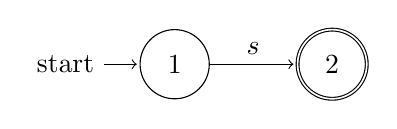
\begin{tikzpicture}[shorten >=1pt,node distance=2cm,on grid,auto] 
       \node[state, initial] (q_1)   {$1$}; 
        \node[state,accepting] (q_2) [ right =of q_1] {$2$};
              
        \path[->] 
        (q_1) edge  node {$s$} (q_2)
        ;
    \end{tikzpicture}
    \caption{$s$}\label{fig:examfignfas}
\end{figure}
Hvis vi sætter figure~\ref{fig:examfignfak}~\ref{fig:examfignfalvh}~\ref{fig:examfignfas} sammen så får vi følgende graf.
\begin{figure}[!ht]
    \centering
    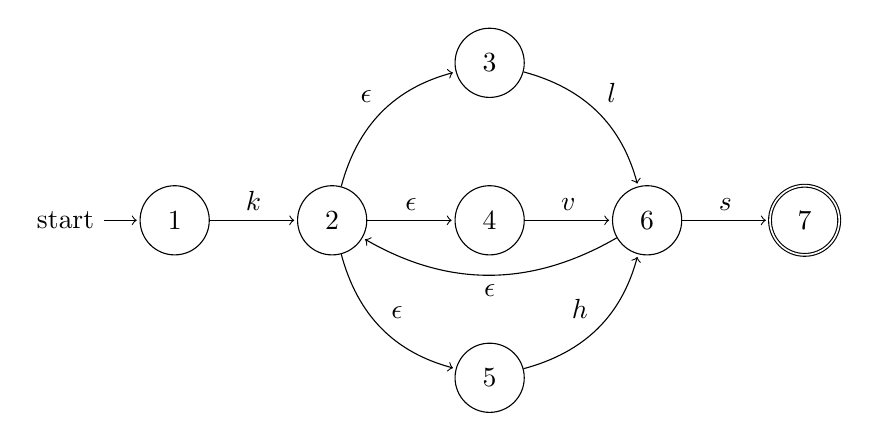
\begin{tikzpicture}[shorten >=1pt,node distance=2cm,on grid,auto] 
        \node[state, initial] (q_1)   {$1$}; 
        \node[state] (q_2) [right=of q_1] {$2$};
        \node[state] (q_4) [ right =of q_2] {$4$};
        \node[state] (q_3) [above  =of q_4] {$3$};
        \node[state] (q_5) [below  =of q_4] {$5$};
        \node[state] (q_6) [right  =of q_4] {$6$};
        \node[state,accepting] (q_7) [ right =of q_6] {$7$};
              
        \path[->] 
        (q_1) edge node{$k$}(q_2)
        (q_2) edge [bend left] node{$\epsilon$}(q_3)
        (q_2) edge node{$\epsilon$}(q_4)
        (q_2) edge [bend right] node{$\epsilon$}(q_5)
        (q_3) edge [bend left] node{$l$}(q_6)
        (q_4) edge node{$v$}(q_6)
        (q_5) edge [bend right] node{$h$}(q_6)
        (q_6) edge node{$s$}(q_7)
        (q_6) edge [bend left=30] node{$\epsilon$}(q_2)
        ;

    \end{tikzpicture}
    \caption{The labeled NFA, representing $k(l|v|h|)+s$}\label{fig:examfignfa}
\end{figure}
\newpage
\subsection{Lav udtrykket om til en DFA}
For at konstruerer en DFA fra NFA'en skal vi inddele automaten i subsæt og se hvilke sæt referer til andre sæt.
\begin{figure}[!ht]
    \centering
    \begin{tabular}{c|cccccc}
            &$k$&$l$&$v$&$h$&$s$&NFA state\\\hline
        $S_1$&$\{2\}^{S_2}$&\{\}&\{\}& \{\}&\{\}& $\{1\}$\\
        $S_2$&\{\}&$\{6\}^{S_3}$&$\{6\}^{S_3}$&$\{6\}^{S_3}$&\{\}&\{2,3,4,5\}\\
        $S_3$&\{\}&$\{\}^{S_3}$&$\{\}^{S_3}$&$\{\}^{S_3}$&$\{7\}^{S_4}$&\{6\}\\
        $S_4$&\{\}&$\{\}$&$\{\}$&$\{\}$&$\{\}$&\{7\}
    \end{tabular}
\end{figure}
Nu kan vi konstruerer DFA'en.
\begin{figure}[!ht]
    \centering
    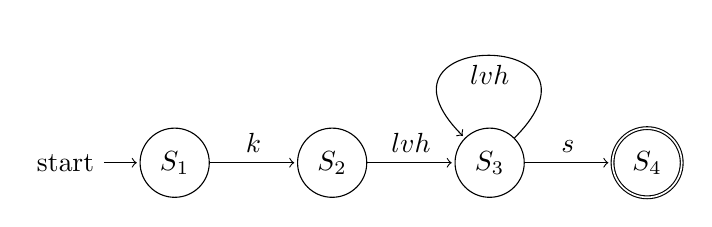
\begin{tikzpicture}[shorten >=1pt,node distance=2cm,on grid,auto] 
        \node[state, initial] (q_1)   {$S_1$}; 
        \node[state] (q_2) [right=of q_1] {$S_2$};
        \node[state] (q_3) [ right =of q_2] {$S_3$};
        \node[state,accepting] (q_4) [ right =of q_3] {$S_4$};
              
        \path[->] 
            (q_1) edge node{$k$}(q_2)
            (q_2) edge  node{$lvh$}(q_3)
            (q_3) edge [loop] node{$lvh$}(q_3)
            (q_3) edge node{$s$}(q_4)
        ;
    \end{tikzpicture}
    \caption{The labeled DFA, representing $k(l|v|h|)+s$}\label{fig:examfigdfa}
\end{figure}
Grunden til at automaten er deterministisk er at der ikke går to ens kanter fra een knude til to forskellige, der eksisterer heller ikke epsilon kanter i automaten angivet i figur~\ref{fig:examfigdfa}.
\subsection{Wtf}
\begin{align*}
    (l+(vl)*(hl)*)|(l*(vl)+(hl)*)|(l*(vl)*(hl)+)
\end{align*}
\section{Opgave 2}
\subsection{Udvid typen expr}
\begin{lstlisting}[style=fsharp]
type expr = 
    ...
    | Ref of expr
    | Deref of expr
    | UpdRef of expr * expr
\end{lstlisting}
\subsection{Udvid typen value}
\begin{lstlisting}[style=fsharp]
type value = 
    | Int of int
    | Closure of string * string * expr * value env
    | RefVal of value ref
\end{lstlisting}
\newpage
\subsection{Udvid eval i higherfun}
Jeg har lavet følgende udvidelse til eval
\begin{lstlisting}[style=fsharp]
let rec eval (e : expr) (env : value env) : value =
    match e with
    ...
    | Ref e -> 
      eval e env |> ref |>  RefVal
    | Deref e -> 
      match eval e env with
      | RefVal v -> v.Value
      | _ -> failwith "You can only dereference reference types"
    | UpdRef(e1, e2) ->
      match eval e1 env with
      | RefVal v -> 
        let other = eval e2 env
        v.Value <- other
        other
      | _ -> failwith "You you tried to update a non reference type"
\end{lstlisting}
beskrivelsen af koden følger:
\begin{itemize}
    \item Ref - Vi evaluerer først udtrykket så vi får en værdi som vi kan putte ind i vores ref celle herefter putter vi den ind i en ref celle så vi ikke længere passerer selve værdien rundt men ene reference til den og til sidst pakker vi den i vore ''RefVal'' type.
    \item Deref - Da vi kun kan hente værdien fra en reference værdi skal vi tjekke om den rent faktisk har den rigtife type, hvis den har det returnere vi værdien, ellers fejler vi.
    \item Updref - Samme som ''Deref'' da vi teknisk set skal ''dereference'' den så vi kan få værdien, forskellen er at vi herefter opdaterer værdien inde i ref cellen, samt returnerer den nye værdi.
\end{itemize}
\begin{lstlisting}[style=fsharp]
let exam2_1 = 
  Let("x", Ref(CstI 2),
    Let("y", Var "x",
      Let("z", UpdRef(Var "y", CstI 42),
          Deref(Var "x")
      )
    )
  )

let exam2_2 = 
  Let("x", Ref(CstB true),
    Deref(Var "x")
  )

let exam2_3 = 
  Let("x", Ref(CstI 10),
    Let("y", Ref(CstI 32),
      Letfun("loop", "i",
        If(
          Prim("=", Deref(Var "x"), CstI 0),
          Deref(Var "y"),
          Let("z", 
            UpdRef(Var "y", 
              Prim("+",
                Deref(Var "y"), 
                CstI 1)
            ),
            Call(Var "loop", UpdRef(Var "x", Prim("-",Deref(Var "x"), CstI 1)))
          )
        ),
        Call(Var "loop", Deref(Var "x"))
      )
    )
  )
let exam2_4 = 
  Let("x", Ref(CstI 1),
    Let("y", Ref(CstI 1),
      UpdRef(Var "x", Prim("+", Deref(Var "x"), Deref(Var "y")))
    )
  )
\end{lstlisting}
\subsection{Udvid lexer og parser}
\begin{lstlisting}[style=fsharp]
{
   let keyword s =
       match s with
       ...
       | "ref"  -> REF
       ...
}
   
   rule Token = parse
     ...
     | ":="            { UPD }
     | '!'             { DEREF }
     ...
\end{lstlisting}
\begin{lstlisting}[style=fsharp]
%token REF UPD DEREF
%left REF              // lowest precedence  
%left ELSE
%left EQ NE UPD
%left GT LT GE LE 
%left PLUS MINUS
%left TIMES DIV MOD 
%nonassoc NOT DEREF          // highest precedence

Expr:
  ...
  | DEREF Expr     { Deref($2)      }
  | REF Expr       { Ref($2)        }
  | Expr UPD Expr  { UpdRef($1, $3) }
;
\end{lstlisting}
I lexeren ``FunLex'' bliver der tilføjet 3 nye tokens, hhv. \Verb|REF|, \Verb|UPD| samt \Verb|DEREF|.\\
I parseren ``FunPar'' bliver de definerede tokens tilføjet samt vurderet præcedens mæssigt. Her har jeg valgt at give \Verb|REF| den laveste præcedens da vi skal kunne definere en værdi med et hvert slags udtryk. Jeg vurderer at \Verb|DEREF| skal have højeste præcedens da man typisk binder den direkte til en variabel, og til sidst har jeg valgt at \Verb|UPD| skal have samme præcedens som \Verb|EQ|.
\subsection{Omskriv eksemplerne}
\begin{lstlisting}[style=fsharp]
let x = ref 1 in 
    if !x = 1 then x := 2 
    else 42 
end
\end{lstlisting}
\begin{lstlisting}[style=fsharp]
let x = ref 2 in 
    (x := 3) + !x 
end
\end{lstlisting}
\begin{lstlisting}[style=fsharp]
let x = ref 10 in 
  let y = ref 32 in
    let loop i =  
        if !x = 0 then !y
        else 
          let z = y := !y+1 in
            loop (x:=!x-1)
          end
      in loop (!x)
    end
  end
end
\end{lstlisting}
\begin{lstlisting}[style=fsharp]
let x = ref 1 in 
  let y = ref 1 in
    x := !x+!y
  end
end
\end{lstlisting}

\end{document}

